% !TeX program = pdflatex
\documentclass[11pt]{amsart}

% Packages
\usepackage[dvipsnames]{xcolor}
\usepackage{enumitem}
\usepackage{amssymb,graphicx,mathtools}
\usepackage{float}
\usepackage{tikz}
\usetikzlibrary{calc,arrows.meta,decorations.markings}
\usepackage[margin=1in]{geometry}
\geometry{letterpaper}
\usepackage{etoolbox}

% Citations
\usepackage[square,longnamesfirst]{natbib}

% Theorem environments, numbered within sections on a shared counter
\theoremstyle{plain}
\newtheorem{theorem}{Theorem}[section]
\newtheorem{proposition}[theorem]{Proposition}
\newtheorem{corollary}[theorem]{Corollary}
\newtheorem{lemma}[theorem]{Lemma}
\theoremstyle{definition}
\newtheorem{remark}[theorem]{Remark}
\newtheorem{problem}{Problem}

% Load hyperref last
\usepackage[
citecolor=PineGreen,
colorlinks=true,
linkcolor=RoyalBlue,
urlcolor=BrickRed
]{hyperref}

\graphicspath{{figures/}}
\allowdisplaybreaks

% Commands
\newcommand{\Z}{\mathbb Z}
\newcommand{\R}{\mathbb R}
\newcommand{\T}{\mathbb T}
\newcommand{\E}{\mathbb E}
\renewcommand{\P}{\mathbb P}
\newcommand{\1}{\mathbf 1}
\newcommand{\ip}[2]{\langle #1,#2\rangle}
\newcommand{\norm}[1]{\lVert #1\rVert}
\newcommand{\abs}[1]{\lvert #1\rvert}
\newcommand{\dd}{\,\mathrm d}
\newcommand{\Hs}{\mathcal H}
\newcommand{\sgn}{\operatorname{sgn}}
\newcommand{\Hminus}[1]{\norm{#1}_{-1,\lambda}}
\newcommand{\Hplus}[1]{\norm{#1}_{1,\lambda}}
\newcommand{\defn}[1]{\textbf{#1}}

% Figure styles
\tikzset{
  ledge/.style={draw=black!22,line width=0.5pt},
  lvert/.style={circle,fill=black,inner sep=1.1pt}
}

\setcounter{secnumdepth}{3}

% No upper case on the title page
\makeatletter
\patchcmd{\@settitle}{\uppercasenonmath\@title}{\Large}{}{}
\patchcmd{\@setauthors}{\MakeUppercase}{\large}{}{}
\makeatother

\title{The randomly oriented Manhattan lattice in 2D is transient}
\author{Ahmed Bou-Rabee}
\author{Yuval Peres}

\begin{document}

\begin{abstract}
Independently orient each horizontal and vertical line of $\Z^2$ by a fair
coin.  A walker chooses one of the two lines through its current position
with equal probability and takes one step in the direction of that line.
Redner \citeyearpar{Red89} introduced this walk as a model of transport in
an isotropic random velocity field and predicted that its root-mean-square
displacement grows like $n^{2/3}$.  We prove that the walk is transient almost
surely.  The proof evaluates an exact variational formula at one explicit
function.
\end{abstract}

\maketitle

\begin{figure}[!b]
\centering
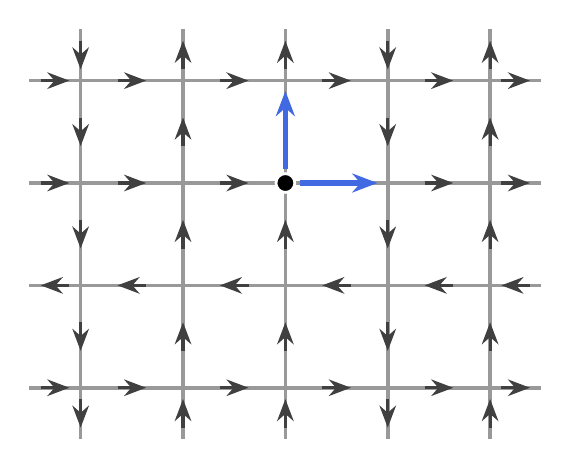
\begin{tikzpicture}[x=1.3cm,y=1.3cm,
  street/.style={draw=black!40,line width=1.3pt},
  head/.style={draw=black!75,line width=1.1pt,-{Stealth[length=2.8mm]}},
  move/.style={draw=RoyalBlue,line width=2.0pt,-{Stealth[length=3.2mm]}},
  site/.style={circle,fill=black,draw=white,line width=1.0pt,inner sep=2.4pt}]
\foreach \y in {0,...,3} \draw[street] (-0.5,\y) -- (4.5,\y);
\foreach \x in {0,...,4} \draw[street] (\x,-0.5) -- (\x,3.5);
% rows 0, 2, 3 run east and row 1 runs west; one head per edge
\foreach \y/\ms in {0/{-0.25,0.5,1.5,2.5,3.5,4.25},
                    2/{-0.25,0.5,1.5,3.5,4.25},
                    3/{-0.25,0.5,1.5,2.5,3.5,4.25}}
  \foreach \m in \ms \draw[head] (\m-0.14,\y) -- (\m+0.14,\y);
\foreach \m in {-0.25,0.5,1.5,2.5,3.5,4.25}
  \draw[head] (\m+0.14,1) -- (\m-0.14,1);
% columns 1, 2, 4 run north and columns 0, 3 run south
\foreach \x/\ms in {1/{-0.25,0.5,1.5,2.5,3.25},
                    2/{-0.25,0.5,1.5,3.25},
                    4/{-0.25,0.5,1.5,2.5,3.25}}
  \foreach \m in \ms \draw[head] (\x,\m-0.14) -- (\x,\m+0.14);
\foreach \x in {0,3} \foreach \m in {-0.25,0.5,1.5,2.5,3.25}
  \draw[head] (\x,\m+0.14) -- (\x,\m-0.14);
\draw[move] (2.14,2)--(2.90,2);
\draw[move] (2,2.14)--(2,2.90);
\node[site] at (2,2) {};
\end{tikzpicture}
\caption{One fair coin directs each line, so every edge of a line points the
same way.  The two blue arrows are the possible steps from the marked site.}
\label{fig:model}
\end{figure}

\section{Introduction}\label{sec:introduction}

The \defn{randomly oriented Manhattan lattice} is the square lattice with
every horizontal and vertical line given a direction by an independent fair
coin.  We study the random walk that at each step chooses one of the two
lines through its position with equal probability and moves one unit in that
line's direction (Figure~\ref{fig:model}).

One coin orients a whole line, so the environment has infinite-range
correlations: whenever the walk returns to a line it has visited before, it is
pushed in the same direction again.  Redner's heuristic in
Section~\ref{sssec:oriented} turns this repetition into the predicted
exponent, and the same feature places the two-dimensional model outside the
general theory recalled in Section~\ref{sssec:divfree}.
Figure~\ref{fig:path} compares the walk with simple random walk at two time
scales.  

\begin{figure}[t]
\centering
\includegraphics[width=0.95\textwidth]{fig_paths.pdf}
\caption{The randomly oriented Manhattan walk on the left and simple random
walk on the right, after $400$ steps in the top row and $4000$ steps in the
bottom row, colored by time from blue to red.  The two panels of each row are
drawn to the same scale.}
\label{fig:path}
\end{figure}

\citet*[p.~290]{Red89} introduced this walk as a model of transport in an
isotropic random velocity field, in work carried out with J.~Koplik,
F.~Leyvraz, and A.~Provata \citep*[p.~287]{Red89}, and predicted that its
root-mean-square displacement grows like $n^{2/3}$.
\citet*[p.~2506]{BGKPR90} subsequently showed that the walk is a random walk
in a divergence-free random velocity field with long-range correlations.
\citet*[Section~1.4]{Tot18} lists this walk among the random walks with
stationary divergence-free drift, and \citet*[Section~3.5]{Pen20} lists the
model among open problems and conjectures the same displacement order
$n^{2/3}$.  Transience was
conjectured by Guillotin-Plantard \citep*[Appendix~A, Conjecture~1]{Bos19},
and \citet*[p.~1]{CHT19} and \citet*[p.~1]{BH23} record it as unresolved.

We prove this conjecture.  The proof starts from an exact variational formula
for the annealed Green function and evaluates it at one function of the
orientations.

\subsection{Main results}\label{ssec:main-results}

Write $e_1$ and $e_2$ for the standard basis vectors of $\Z^2$.  Every line
of $\Z^2$ parallel to $e_1$ or to $e_2$ is given a direction by an
independent fair coin.  Record these choices in a function
$\omega\colon\Z^2\times\{1,2\}\to\{-1,1\}$, where $\omega(z,i)=1$ if the line
through $z$ parallel to $e_i$ points along $e_i$, and $\omega(z,i)=-1$
otherwise.  That line is unchanged when $z_i$ varies, so $\omega(z,i)$ does
not depend on $z_i$.  We call $\omega$ the \defn{environment} and write $\P$
for its law.

From $z$ the walker steps to
\begin{equation}\label{eq:rule}
  z+\omega(z,1)e_1\qquad\text{or}\qquad z+\omega(z,2)e_2,
  \qquad\text{with probability $1/2$ each.}
\end{equation}
Because $\omega(z,i)$ does not
depend on $z_i$, it agrees with $\omega(z-e_i,i)$, so the drift $\omega$ has
vanishing discrete divergence.  Every site therefore has two incoming and two
outgoing directed edges, and counting measure is invariant.

Write $P^\omega_z$ for the quenched law of the walk started at $z$ in a fixed
environment $\omega$, and write $p^\omega_n(z,z')$ for the probability under
$P^\omega_z$ that the walk is at $z'$ after $n$ steps.
Averaging over $\omega$ gives the annealed transition probability
$\overline p_n(z,z')=\E p^\omega_n(z,z')$.

\begin{theorem}\label{thm:main}
For $\P$-almost every environment $\omega$,
\[
  \sum_{n\geq0}p^\omega_n(x,x)<\infty\qquad\text{for every }x\in\Z^2\, .
\]
That is, the walk is transient in almost every environment.
\end{theorem}

We deduce Theorem~\ref{thm:main} from an annealed bound in continuous time.
Consider the continuous-time walk that jumps from $z$ to $z+\omega(z,i)e_i$
at rate $1$, for $i=1$ and $i=2$.  Its total jump rate is $2$, and its jump
chain is the walk in \eqref{eq:rule}.  Write
$p^\omega_t(z,z')$ for its transition probabilities and set
$\overline p_t(0,0)=\E p^\omega_t(0,0)$.

\begin{theorem}\label{thm:annealed}
There is a constant $C<\infty$ with
\[
  \int_0^\infty e^{-\lambda t}\overline p_t(0,0)\dd t\leq C
  \qquad\text{for all }\lambda\in(0,1]\, ,
\]
and hence $\int_0^\infty\overline p_t(0,0)\dd t<\infty$.
\end{theorem}

The continuous-time generator is the centered finite-difference
analogue of diffusion with drift: for every $h\colon\Z^2\to\R$,
\begin{equation}\label{eq:discrete-drift}
\begin{split}
  (\mathcal G_\omega h)(z)
  &=\frac12\sum_{i=1}^2
    \bigl[h(z+e_i)+h(z-e_i)-2h(z)\bigr]\\
  &\quad+\frac12\sum_{i=1}^2\omega(z,i)
    \bigl[h(z+e_i)-h(z-e_i)\bigr]\, .
\end{split}
\end{equation}
The first line is the symmetric simple-random-walk generator.  The second is
the centered first difference with coefficient $\omega$, and the vanishing
divergence noted above is its discrete incompressibility condition.

The randomness is essential.  Take instead the alternating orientations,
$\omega(z,1)=(-1)^{z_2}$ and $\omega(z,2)=(-1)^{z_1}$.  Then the
position at an even time, with each coordinate halved and rounded down,
performs simple random walk on $\Z^2$, so the walk is recurrent.  \citet*[p.~2]{BH23} report
this and attribute it to Guillotin-Plantard.

Equation~\eqref{eq:discrete-drift} also gives the comparison with a Brownian
particle in an incompressible random drift.  In the $d$-dimensional version,
the covariance of one component of $\omega$ is supported on its coordinate
axis.  Its average over a box of side $R$ has order $R^{1-d}$.  The average
over the same box of an isotropic covariance of order
$\abs{x-y}^{-2(1-\gamma)}$, as in \citet*[(1.2)]{ABK26}, has order
$R^{-2(1-\gamma)}$.  Matching these powers gives the heuristic
correspondence
\begin{equation}\label{eq:gamma-dimension}
  \gamma=\frac{3-d}{2}\, .
\end{equation}
Under this correspondence, the renormalization-group prediction
\citep*[(1.3)]{ABK26} gives variance of order $t^{4/3}$ in dimension two,
$t(\log t)^{1/2}$ in dimension three, and $t$ in dimensions at least four.
These are also the three regimes of the $\Hs_{-1}$ condition recorded in
\citet*[Section~1.4]{Tot18}.  We prove transience in dimension two by choosing
an explicit function in a variational formula for the Green function.

\subsection{Related work}\label{ssec:related-work}

\subsubsection{Random walks on oriented lattices}\label{sssec:oriented}

Redner obtained the exponent $\nu=2/3$ by the following heuristic self-consistency argument \citep*[p.~290]{Red89}.  Suppose that the   horizontal displacement by time $t$ has scale $R=R(t)$. Of the $R$ vertical lines the walk encounters, about half point up and half down, but there is typically a surplus of order $\sqrt{R}$ in one of these directions. Since each of these lines is visited    $t/R$ times on average, this yields an expected vertical displacement  of order $t/\sqrt{R}$. Isotropy of the model then yields  $t/\sqrt{R} \approx R$, so $R \approx t^{2/3}$. 
 
In dimension $d$, the lines in one coordinate direction are indexed by
$d-1$ transverse coordinates.  The analogous volume count uses
$R(t)^{d-1}$ independent orientations and gives
\[
  R(t)\asymp tR(t)^{-(d-1)/2},
  \qquad\text{hence}\qquad
  \nu=\frac{2}{d+1}\, .
\]
Redner states this power-law prediction for $d\leq3$.
\citet*[p.~152, item~\textup{(v)} and (1.73a)--(1.73b)]{BG90} give the same
two-dimensional calculation and describe the model as following Redner.

In dimensions two and three, \citet*[Theorem~1.1 and the discussion following
it]{LTV18} proved two-sided bounds on the Laplace transform of the mean-square
displacement.  They also recorded the predicted orders
$t^{4/3}$ in dimension two and $t(\log t)^{1/2}$ in dimension three.  
\citet*[Theorem~1.1]{Ngu26} recently presented a deep analysis of the three-dimensional case. He proved that, for every $\varepsilon>0$ and all
sufficiently small $\lambda$,   this Laplace transform  is of order
$\lambda^{-2}\sqrt{\abs{\log\lambda}}$,
up to a multiplicative factor
$(\log\abs{\log\lambda})^{\pm(2+\varepsilon)}$.  This answers a conjecture of
\citet*{LTV18} in the critical dimension.  


In the singly oriented analogue only the horizontal lines are directed, and
the vertical coordinate performs an autonomous random walk.  This model
originates in the work of \citet*{MdM80}; see also
\citet*[pp.~2--3]{LTV18}.  For this model, \citet*[Theorem~20]{CGPS11} proved a local limit
theorem  and obtained return probability of order $n^{-5/4}$.  Their
argument uses the autonomous vertical walk. For the randomly oriented Manhattan lattice, simulations of \citet*[Section~3.2]{MNOV20} indicate a return probability of
order $n^{-4/3}$.

For  the classical Manhattan lattice with  alternating deterministic orientations, \citet*[Theorem~1]{BH23}
computed exactly the mean-square displacement.    That walk is
diffusive and recurrent, as recalled in Section~\ref{ssec:main-results}, so randomizing the orientations turns a recurrent walk into a transient one.  If a walker at $z$ instead moves deterministically to
$z+\omega(z,1)e_1+\omega(z,2)e_2$ at every step, then
\citet*[Theorem~1]{CHT19} proved that its trajectory is eventually
two-periodic.
\citet*[pp.~10251--10254]{BOC03}
study quantum and classical network models embedded in the deterministic
Manhattan lattice.

\subsubsection{Divergence-free drifts}\label{sssec:divfree}

Our walk belongs to the class of random walks in stationary doubly
stochastic environments; double stochasticity is the invariance of counting
measure noted above.
Under the annealed law, the environment seen from the walker is stationary
and ergodic.  \citet*[Sections~1.1--1.2]{Tot18} treats these walks together
with diffusions in stationary incompressible random flows.

The $\Hs_{-1}$ condition asks that the drift covariance be integrable at low
frequencies.  It is equivalent to writing the drift as the divergence of a
stationary square-integrable antisymmetric matrix field, called its stream
matrix \citep*[Proposition~1\textup{(ii)}]{Tot18}.  Under
double stochasticity, zero annealed drift, ellipticity of the symmetric
rates, and the $\Hs_{-1}$ condition, \citet*[Theorem~1]{KT17} proved a central
limit theorem: the diffusively rescaled finite-dimensional distributions
converge to Brownian motion in probability with respect to the environment.  Under the additional
$L^{2+\varepsilon}$ integrability assumption on the stream matrix,
\citet*[Theorem~1\textup{(ii)}]{Tot18Q} proved the quenched central limit
theorem.  For the randomly oriented Manhattan lattice, the $\Hs_{-1}$
condition fails with a power-law divergence in dimension two, fails
logarithmically in dimension three, and holds in dimensions at least four
\citep*[Section~1.4]{Tot18}.  The theorems just quoted therefore do not apply
in dimensions two and three.

The continuum counterpart is a diffusion in an incompressible random drift.
Equation~\eqref{eq:discrete-drift} is the centered finite-difference version
of $\nu\Delta+f\cdot\nabla$ with $\nu=1/2$.  That operator generates
$\dd X_t=f(X_t)\dd t+\sqrt{2\nu}\dd W_t$
\citep*[(1.1)]{ABK26}.  An incompressible continuum drift is
written as $f=\nabla\cdot k$ for a stream matrix $k$, so its
generator is $\nabla\cdot(\nu I+k)\nabla$
\citep*[(1.9)]{ABK26}.  The same divergence-form operator appears in
\citet*[Theorem~1 and (1.2)--(1.5)]{Oel88}, who proved homogenization under
the square-integrability, regularity, and growth assumptions stated there.

For the Manhattan walk, define the discrete stream function by
\begin{equation}\label{eq:stream}
  \psi^\omega(z+e_2)-\psi^\omega(z)=\omega(z,1),
  \qquad
  \psi^\omega(z+e_1)-\psi^\omega(z)=-\omega(z,2),
  \qquad \psi^\omega(0)=0\, .
\end{equation}
Then $\omega$ is the rotated discrete gradient of $\psi^\omega$.  Along
each coordinate, $\psi^\omega$ is a sum of independent signs.  Formally
replacing these two random-walk partial sums by their Brownian scaling limits
gives
\[
  \psi(x,y)=W_1(y)-W_2(x),
  \qquad f=(\partial_y\psi,-\partial_x\psi)\, .
\]
Thus the two components of $f$ are constant along horizontal and vertical
lines, respectively, just as in the lattice model.

For the curl of the two-dimensional Gaussian free field,
\citet*[Theorem~1 and Remark~2]{TV12} proved superdiffusivity, with
Laplace-transform bounds corresponding to $t\log\log t$ and $t\log t$, and
predicted the order $t(\log t)^{1/2}$.
\citet*[Theorem~1.1]{CMOW25} proved that the mean-square displacement is of
that order.  \citet*[Theorem~A]{ABK24} proved a quenched invariance principle
at this scaling, and identified the leading constant, for drifts whose
covariance decays like $\abs{x-y}^{-2}$;
their equation~(1.3) predicts diffusive behavior for faster covariance decay
and superdiffusive behavior for slower decay.
\citet*[Theorem~A]{ABK26} proved quenched power-law superdiffusion, with
displacement variance of order $t^{2/(2-\gamma)}$, for a stream matrix of
sufficiently small Hurst exponent $\gamma>0$.
\citet*[Section~1.2]{ABK24} allows multiscale log-correlated, non-Gaussian
stream matrices and includes the mollified Gaussian free field.
\citet*[Section~1.5]{ABK26} instead assumes independent finite-range stream
increments at successive scales.  The stream function in
\eqref{eq:stream} has independent $\pm1$ increments along the two coordinate
axes.

\subsubsection{The variational formula}\label{sssec:variational}

When a diffusion in a divergence-free random flow rescales to a Brownian
motion, the covariance of that Brownian motion is called the effective
diffusivity.  Variational formulas for it are standard in homogenization.
\citet*[Section~V.1, (5.20)]{AM91} give a minimum principle for it, nonlocal
because a projection appears in the functional.
\citet*[Section~4.1, (4.22) and (4.43)--(4.44)]{FP96} derive a min--max
principle for a stationary random flow, together with the minimum and maximum
principles that follow from it.  Working on the probability space of the flow
rather than on space, \citet*[Proposition~5.1, (5.1)--(5.2)]{LOY98} give a
matching pair of supremum and infimum formulas.

Our walk has no diffusive limit, so we use the analogue of these formulas
for the resolvent at a positive $\lambda$ rather than for the limit
$\lambda\to0$.  For a generator $L=S+A$ with $S$ self-adjoint and $A$
skew-adjoint, \citet*[Theorem~4.1]{KLO12} express
$\operatorname{Re}\ip V{(\lambda I-L)^{-1}V}$ as an infimum of a quadratic
functional; the domain condition in that theorem is automatic here, because
the operators in this paper are bounded.  Closely related resolvent formulas
appear in \citet*[(2.17)]{LQSY04} and \citet*[(39)]{Tot18}, and
\citet*[Theorem~2.4 and Section~2.3]{GL14} prove the corresponding statement
for capacities of nonreversible Markov chains.

The same quadratic functional appears in quantitative homogenization, where
it is used to bound the effective diffusivity of a divergence-form operator.
\citet*[Exercise~10.1, immediately before (10.13)]{AKM19} record it for a
general coercive nonsymmetric bilinear form; taking that form to be
$\operatorname{Re}\ip v{(H+A_p)u}$, twice their functional at $(g,1)$ is the
expression in \eqref{eq:overview-bound}.  For symmetric coefficients
the corresponding pair is the Dirichlet energy and its convex dual, in
\citet*[(2.1)--(2.2)]{AS16} and \citet*[(2.6)--(2.9)]{AKM19}.  For
incompressible random drifts, \citet*[(2.4)--(2.5)]{ABK24} and
\citet*[(2.32)--(2.37)]{ABK26} take infima and suprema over a box to define a
diffusivity matrix at each scale.  Those works compare the variational quantities at
successive scales.  Here we evaluate the resolvent formula directly at one
function.

\subsection{Proof overview}\label{ssec:proof-overview}

Transience follows from the finiteness of the annealed Green function in
Theorem~\ref{thm:annealed}.  For a reversible walk such a bound is classically
obtained by exhibiting a unit flow of finite energy; see
e.g.\ \citet*[Theorem~2.11]{LP16}.  That criterion is usable because no
optimal flow is needed: any flow of finite energy gives the conclusion.  Our
walk is not reversible, so the criterion does not apply, but the argument
below has the same shape.  An exact variational
formula expresses the quantity to be bounded as a minimum over functions of
the orientations, and exhibiting a single such function bounds it.

The environment is invariant under translations of $\Z^2$, so a Fourier
transform in the position variable decomposes the Green function into an
integral over $p\in\T^2$ of resolvents $r_\lambda(p)$, one for each frequency,
and it suffices to bound these separately.  At a fixed $p$, split the
generator into a self-adjoint part $S_p$ and a skew-adjoint part $A_p$, and
put $H=\lambda I-S_p$.  Theorem~4.1 of \citet*{KLO12}, applied on the
underlying real Hilbert space, gives the exact identity
\begin{equation}\label{eq:overview-bound}
  r_\lambda(p)=\inf_g\left\{
  \ip g{Hg}+\ip{1-A_pg}{H^{-1}(1-A_pg)}\right\}\, .
\end{equation}
Every $g$ is a competitor in this infimum and gives an upper bound, so the
proof consists of choosing one.  The first term measures the cost of $g$, the
second the failure of $A_pg$ to equal the constant $1$; a good choice makes
$A_pg$ nearly constant without paying much for it, in the way a good flow
carries a unit of current at small energy.

A function of the orientations depends on the infinitely many independent
signs carried by the lines, and expands in products of distinct signs, the
analogue of a Fourier series for coin flips.  Call the number of signs in a
product its degree.  Multiplying by one
orientation adds or removes a single sign, so $A_p$ carries each degree to
its two neighbours.  The constant $1$ in \eqref{eq:overview-bound} has degree
zero, so a competitor must have a degree-one part to meet it; that part then
leaves an error of degree two, which a degree-three part can cancel.  The
three steps below carry this out.

\medskip

\noindent\textbf{Step 1.}  Work in these coordinates.  Products of distinct
signs are orthogonal and $H$ preserves the degree, so both terms in
\eqref{eq:overview-bound} split into separate contributions from each degree.
Take $g$ with components of degrees one and three.

\medskip

\noindent\textbf{Step 2.}  Suppose $\abs{p_1}\geq\abs{p_2}$, and let $K$ be
large and $r_0$ small, both fixed in \eqref{eq:params}.  Set
\[
  a=\abs{p_1},\qquad
  L=1+\log_+\frac{r_0}{\sqrt\lambda+a}\, .
\]
The degree-one component $f_p$ is supported on the frequency interval
$[K(\sqrt\lambda+a),r_0]$, where it is proportional to $1/\sin r$.  Each
dyadic range of frequencies inside that interval then contributes the same
amount to the constant component $b_p$ of $A_pf_p$, and $L$ counts those
ranges, so $b_p\geq caL$.  The logarithms in the bounds below all come from
this count.  Apart from a term of bounded $H^{-1}$ norm, the rest of $A_pf_p$
is the indicator function of that interval.

\medskip

\noindent\textbf{Step 3.}  Choose the degree-three component $k_p$ by
minimizing the part of \eqref{eq:overview-bound} that contains this
indicator.  The minimization decouples into a scalar problem at each pair of
frequencies, and the denominator of its solution carries a logarithm of its
own.  Integrating that solution gives
\begin{equation}\label{eq:overview-estimates}
  E_p(f_p,k_p)\leq C\sqrt L\, ,
\end{equation}
where $E_p$, defined in \eqref{eq:E}, is the sum of the first term in
\eqref{eq:overview-bound} and the nonconstant part of the second.

Now take $g=(f_p+k_p)/b_p$.  Its constant component cancels the $1$ in
\eqref{eq:overview-bound}, and orthogonality gives
\[
  \ip g{Hg}+\ip{1-A_pg}{H^{-1}(1-A_pg)}
  =E_p(f_p,k_p)/b_p^2\, ,
\]
and hence
\[
  r_\lambda(p)\leq\frac{E_p(f_p,k_p)}{b_p^2}
  \leq\frac C{a^2L^{3/2}}\, .
\]

Three choices of $g$ are worth comparing.  Taking $g=0$ gives the bound for
the walk with no drift, of order $a^{-2}$ at small frequencies, and its
integral near the origin diverges logarithmically as $\lambda\to0$; that
divergence is the recurrence of two-dimensional simple random walk.  A
competitor of degree one alone gives $a^{-2}L^{-1}$, and the choice above
gives $a^{-2}L^{-3/2}$.  Substituting $u=\log(r_0/a)$ turns the frequency
integral near the origin into $\int_1^\infty u^{-1}\dd u$ for the degree-one
bound, which diverges, and $\int_1^\infty u^{-3/2}\dd u$ for the last, which
converges.  The gain of $\sqrt L$ from the degree-three part therefore decides
the theorem.  Taking the minimum of the last bound with the driftless one
gives a function of $p$ that is integrable uniformly in $\lambda$, which
proves the annealed Green-function bound.  Running the discrete walk with a
rate-two Poisson clock gives the continuous-time walk, whose Green function is
half the discrete one, so Theorem~\ref{thm:main} follows.
Sections~\ref{sec:variational}--\ref{sec:evaluation} carry out this
construction, and Section~\ref{sec:calculations} proves the
operator estimates used in its evaluation.

\subsection{Notation and conventions}\label{ssec:notation}

\begin{itemize}
\item All torus integrals use the normalized Haar measure
$\dd m(s)=\dd s/2\pi$ on $\T=(-\pi,\pi]$, and $\dd m(p)=\dd m(p_1)\dd m(p_2)$
on $\T^2$.
\item $\ip\cdot\cdot$ and $\norm\cdot$ are the real or complex $L^2$ inner
product and norm on the space under discussion.
\item $c>0$ and $C>0$ denote finite constants whose value may change from
line to line and is never tracked.  Constants that must be held fixed are
given their own names.
\end{itemize}

\section*{Acknowledgments}
The research of Y. Peres was supported by National Natural Science Foundation of China grant
RFIS-W2531011.  We acknowledge use of ChatGPT 5.6.

\section{The variational formula}\label{sec:variational}

We first write the annealed Green function as an integral of fixed-frequency
resolvents.  The variational formula then reduces the proof to the
construction of one competitor at each frequency.

\subsection{Fourier transform}\label{ssec:fourier}

Recall from Section~\ref{ssec:main-results} that $\omega(z,i)$ does not
depend on $z_i$.  For
$x\in\Z^2$, define
\[
  (T_xF)(\omega)=F(\tau_x\omega),
  \qquad (\tau_x\omega)(z,i)=\omega(z+x,i)\, .
\]
The operator $T_x$ is unitary on $L^2(\P)$, and $T_{\pm e_i}$ commutes with
multiplication by $\omega(0,i)$.

On $L^2(\P;\ell^2(\Z^2))$, regard $\delta_0$ as the function
$\delta_0(\omega,z)=\1_{\{z=0\}}$.  The environment seen
from the walk, paired with the position of the walk, has generator
\begin{equation}\label{eq:joint-generator}
  (\mathcal GF)(\omega,z)=\sum_{i=1}^2
  \bigl[F(\tau_{\omega(0,i)e_i}\omega,z+\omega(0,i)e_i)-F(\omega,z)\bigr]\, .
\end{equation}
Starting from $(\omega,0)$, its second component is the position of the
walk.  Therefore
\begin{equation}\label{eq:return-correlation}
  \overline p_t(0,0)=\ip{\delta_0}{e^{t\mathcal G}\delta_0}\, .
\end{equation}

For $F\in L^2(\P;\ell^2(\Z^2))$, take the Fourier transform
$\widehat F(\omega,p)=\sum_{z\in\Z^2}e^{-ip\cdot z}F(\omega,z)$.  Under this
transform, $F(\tau_x\omega,z+x)$ becomes $e^{ip\cdot x}T_x\widehat F$.
Consequently, $\mathcal G$ becomes the family $G_p=S_p+A_p$ below.  At
$p=0$ these are the operators $S$ and $A$ of \citet*[(1.5)--(1.6)]{LTV18}, and
the Hilbert-space facts recorded below are those of
\citet*[Section~2]{KT17}, whose proofs use only the unitarity of the shifts.

\begin{proposition}\label{prop:generator}
For each $p\in\T^2$, the operator $G_p$ equals $S_p+A_p$, where
\begin{align}
  S_p&=\frac12\sum_{i=1}^2
  \bigl(e^{ip_i}T_{e_i}+e^{-ip_i}T_{-e_i}-2I\bigr),\label{eq:Sp}\\
  A_p&=\frac12\sum_{i=1}^2\omega(0,i)
  \bigl(e^{ip_i}T_{e_i}-e^{-ip_i}T_{-e_i}\bigr)\, .\label{eq:Ap}
\end{align}
The operator $S_p$ is self-adjoint and nonpositive, $A_p^*=-A_p$,
$\norm{S_p}\leq4$, and $\norm{A_p}\leq2$.  Put
\[
  d(s)=1-\cos s,\qquad
  \theta(p)=d(p_1)+d(p_2)\, .
\]
For every $\lambda>0$,
\begin{align}
  \int_0^\infty e^{-\lambda t}\overline p_t(0,0)\dd t
      &=\int_{\T^2}r_\lambda(p)\dd m(p),\label{eq:green}\\
  r_\lambda(p)&\coloneqq
      \operatorname{Re}\ip 1{(\lambda I-G_p)^{-1}1}\, .\label{eq:frequency-resolvent}
\end{align}
\end{proposition}

\begin{proof}
Splitting each summand of \eqref{eq:joint-generator} into the two possible
values of $\omega(0,i)$ gives \eqref{eq:Sp} and \eqref{eq:Ap}.  Each
$e^{ip_i}T_{e_i}$ is unitary and commutes with multiplication by
$\omega(0,i)$, so the assertions about $S_p$ and $A_p$ follow as in
\citet*[Section~2]{KT17}.  The Fourier transform of $\delta_0$ is the constant
function $1$, so Plancherel's theorem and the resolvent identity applied to
\eqref{eq:return-correlation} give \eqref{eq:green} and
\eqref{eq:frequency-resolvent}.
\end{proof}

\subsection{The fixed-frequency formula}\label{ssec:varbound}

Fix $p\in\T^2$ and write
\begin{equation}\label{eq:H}
  H\coloneqq\lambda I-S_p,
  \qquad \lambda I\leq H\leq(\lambda+4)I,
  \qquad H1=(\lambda+\theta(p))1\, .
\end{equation}
Thus $H^{-1}$ and $H^{-1/2}$ are bounded.  Use the standard $H^{\pm1}$
norms
\begin{equation}\label{eq:Hnorms}
  \Hplus g^2\coloneqq\ip g{Hg},
  \qquad
  \Hminus u^2\coloneqq\ip u{H^{-1}u}\, .
\end{equation}

Regard the complex space $L^2(\P)$ as a real Hilbert space with inner product
$\operatorname{Re}\ip\cdot\cdot$.  Since $G_p$ is bounded, condition~(4.2)
of \citet*{KLO12} is automatic.  Their Theorem~4.1, applied to $G_p$ with
$V=1$, and then with $g$ replaced by $-g$, gives
\begin{equation}
  r_\lambda(p)
  =\inf_g\Bigl\{\Hplus g^2+\Hminus{1-A_pg}^2\Bigr\}\, .
  \label{eq:var}
\end{equation}
For capacity, the corresponding nonreversible Dirichlet principle is
\citet*[Theorem~2.4 and (2.9)--(2.10)]{GL14}.
The infimum is over complex functions in $L^2(\P)$.  We use the formula only
by substitution: every competitor gives an upper bound for $r_\lambda(p)$.

\subsection{The frequency bound}\label{ssec:frequency}

The proof of transience reduces to the following estimate.

\begin{proposition}\label{prop:frequency}
There are constants $r_0\in(0,1)$ and $C<\infty$ such that, for every
$\lambda\in(0,1]$ and $p\in\T^2$, if
\[
  a(p)=\max\{\abs{p_1},\abs{p_2}\},
  \qquad L_\lambda(p)=1+\log_+\frac{r_0}{\sqrt\lambda+a(p)}\, ,
\]
then there is $g_{\lambda,p}\in L^2(\P)$ such that
\begin{equation}\label{eq:frequency-bound}
  \Hplus{g_{\lambda,p}}^2+
  \Hminus{1-A_pg_{\lambda,p}}^2
  \leq C\min\left\{
  \frac1{\lambda+\theta(p)},
  \frac1{a(p)^2L_\lambda(p)^{3/2}}
  \right\}\, ,
\end{equation}
where the second entry is $+\infty$ when $a(p)=0$.
\end{proposition}

Sections~\ref{sec:coins} and~\ref{sec:evaluation} prove
Proposition~\ref{prop:frequency} by evaluating the right side of
\eqref{eq:var} at one function with components of degrees one and
three.

\begin{proof}[Proof of Theorem~\ref{thm:annealed} given Proposition~\ref{prop:frequency}]
By Proposition~\ref{prop:generator}, \eqref{eq:var}, and
Proposition~\ref{prop:frequency}, it suffices to integrate the right side of
\eqref{eq:frequency-bound}.  On $\{a(p)\leq\sqrt\lambda\}$, use the first entry;
this region has measure $O(\lambda)$ and its contribution is $O(1)$.  On
$\{\sqrt\lambda<a(p)<r_0/2\}$, use the second entry and square annuli to get
\[
  C\int_{\sqrt\lambda}^{r_0/2}
  \frac{\dd a}{a[1+\log(r_0/2a)]^{3/2}}
  \leq C\int_1^\infty\frac{\dd u}{u^{3/2}}<\infty\, .
\]
On $\{a(p)\geq r_0/2\}$, use the first entry and
$\theta(p)\geq c(r_0)$.  This bounds the left side of \eqref{eq:green} by $C$.  Monotone
convergence in \eqref{eq:green} gives
$\int_0^\infty\overline p_t(0,0)\dd t<\infty$.
\end{proof}

\begin{proof}[Proof of Theorem~\ref{thm:main} given Theorem~\ref{thm:annealed}]
Theorem~\ref{thm:annealed} and Tonelli's theorem give
$\int_0^\infty p_t^\omega(0,0)\dd t<\infty$ for almost every $\omega$.  If
$N_t$ is an independent rate-two Poisson process, then the continuous-time
walk at time $t$ is the discrete-time walk after $N_t$ steps, and
\[
  \int_0^\infty p_t^\omega(0,0)\dd t
  =\frac12\sum_{n\geq0}p_n^\omega(0,0)\, .
\]
Thus the sum on the right is finite almost surely.  Finally,
$p_n^\omega(x,x)=p_n^{\tau_x\omega}(0,0)$ and $\P$ is translation invariant.
Intersecting the probability-one events over $x\in\Z^2$ proves the theorem.
\end{proof}

We now prove Proposition~\ref{prop:frequency}.

\section{Fourier--Walsh coordinates}\label{sec:coins}

Fix $p\in\T^2$ and write $A=A_p$.  Choosing $g$ in \eqref{eq:var} calls for
coordinates in which the two quadratic terms can be estimated separately.
The orientations are independent signs, so products of signs form an
orthonormal basis, and grading by the number of signs in a product
diagonalizes $H$ while $A$ shifts the grading by one.  This section records
the resulting formulas and restricts the objective to the two degrees the
construction uses.

Products of distinct independent signs form an orthonormal basis for
functions of finitely many signs.  Conditional expectation onto increasing
finite sets of signs and $L^2$ martingale convergence extend this basis to
$L^2(\P)$; see \citet*[Theorem~1.5]{ODo14} for the finite-dimensional
Fourier--Walsh expansion.

\subsection{Degree and frequency}\label{ssec:degree}

Index each line sign by $(x,j)$, where $j\in\{1,2\}$ and
$x\in\{z\in\Z^2:z_j=0\}$.  A sign of type $1$ is a row sign,
and a sign of type $2$ is a column sign.  Let $\Hs_n$ be the closed span of
products of $n$ distinct line signs.  Every $F\in\Hs_n$ has a symmetric
coefficient $f$ such that
\[
  F(\omega)=\sum_{\mathbf x,\mathbf j}f_{\mathbf j}(\mathbf x)
  \prod_{a=1}^n\omega(x_a,j_a)\, ,
\]
where $f$ vanishes when two line indices coincide.  If $F\in\Hs_n$ and
$G\in\Hs_m$ have coefficients $f$ and $g$, then
\begin{equation}\label{eq:iso}
  \ip FG=\1_{\{m=n\}}n!\ip fg_{\ell^2}\, .
\end{equation}

Multiplication by $\omega(0,i)$ adds the corresponding line sign when it is
absent and removes it when it is present.  Consequently
\begin{equation}\label{eq:DA}
  A=D-D^*,\qquad D\colon\Hs_n\longrightarrow\Hs_{n+1}\, .
\end{equation}
Let $\Pi_n$ denote the orthogonal projection onto coefficients supported on
distinct line indices.
Write $H_n$ for the restriction of $H$ to $\Hs_n$.

Take Fourier series in the line indices and drop the hats.  A line frequency
$q$ of type $j$ satisfies $q_j=0$.  For a degree-$n$ coefficient, put
\begin{equation}\label{eq:P}
  P=p+q_1+\cdots+q_n\, .
\end{equation}
Equations~\eqref{eq:Sp} and \eqref{eq:H} give
\begin{equation}\label{eq:Hsym}
  \text{$H_n$ is multiplication by }\lambda+\theta(P)\, .
\end{equation}
We also use
\begin{equation}\label{eq:sine}
  \log_+x=\max\{0,\log x\},
  \qquad \frac{2s^2}{\pi^2}\leq d(s)\leq\frac{s^2}{2}
  \quad (\abs s\leq\pi)\, .
\end{equation}
In degree zero, \eqref{eq:Hsym} reads $H_0=\lambda+\theta(p)$.

\subsection{Degrees one and three}\label{ssec:degrees-one-three}

Restricting the objective in \eqref{eq:var} to the two degrees we use gives a
quadratic form in their coefficients.  For $f\in\Hs_1$ and $k\in\Hs_3$,
define
\begin{equation}\label{eq:E}
  E_p(f,k)=\ip f{H_1f}+\ip k{H_3k}
  +\Hminus{D_1f-D_2^*k}^2+\Hminus{D_3k}^2\, .
\end{equation}
If $D_0^*f=-b$ with $b>0$, the degree-zero part of
$A(f+k)$ is $b$.  Orthogonality of the Walsh degrees therefore gives
\begin{equation}\label{eq:exact-cancellation}
  \Hplus{\frac{f+k}{b}}^2+
  \Hminus{1-A\frac{f+k}{b}}^2
  =\frac{E_p(f,k)}{b^2}\, .
\end{equation}
The zero function gives
\begin{equation}\label{eq:zero-function}
  \Hplus0^2+\Hminus1^2=\frac1{\lambda+\theta(p)}\, .
\end{equation}
It remains to prove the following two estimates.  After exchanging rows and
columns, suppose
$\abs{p_1}\geq\abs{p_2}$, put $a=\abs{p_1}$, and let
$L=L_\lambda(p)$.  When $L$ is larger than a fixed constant, we construct
$f_p\in\Hs_1$ and $k_p\in\Hs_3$ such that
\begin{equation}\label{eq:construction}
  D_0^*f_p=-b_p,\qquad b_p\geq caL,\qquad
  E_p(f_p,k_p)\leq C\sqrt L\, .
\end{equation}
The coefficient $f_p$ contains one row sign, and $k_p$ contains two row
signs and one column sign.

\subsection{Low-degree coordinates}\label{ssec:low-coordinates}

Only degrees one and three occur, with at most one column sign.  A row sign
has frequency $q=(0,s)$ and a column sign has frequency
$q=(u,0)$.  In place of $s$ and $u$ we always use the shifted variables
\begin{equation}\label{eq:shift}
  r=p_2+s,\qquad r'=p_2+s',\qquad \beta=p_1+u,
  \qquad\text{and}\qquad \alpha=r+r'-p_2\, .
\end{equation}
In these variables the total frequency of each coefficient type is written
with one letter per line sign,
\[
\renewcommand{\arraystretch}{1.15}
\begin{array}{llll}
  \text{degree $0$:} & P=(p_1,p_2), &\quad
  \text{two rows:} & P=(p_1,\alpha),\\
  \text{one row:} & P=(p_1,r), &\quad
  \text{mixed:} & P=(\beta,r),\\
  & &\quad \text{two rows and a column:} & P=(\beta,\alpha)\, .
\end{array}
\]
The letter $\alpha$ has to be $r+r'-p_2$ because each of $r$ and $r'$ already
contains one copy of $p_2$.  Since $p$ is frozen, $\dd m(s)=\dd m(r)$ and
$\dd m(u)=\dd m(\beta)$, so no Jacobian appears.  Every formula below uses
the shifted variables \eqref{eq:shift}.

\subsection{Low-degree operators}\label{ssec:low-operators}

We need only the following actions of $D$ and $D^*$.

Because of the factor $n!$ in \eqref{eq:iso}, multiply the coefficients of
types $11$, $12$, and $112$ by
$\sqrt2$, $2$, and $\sqrt{18}$, respectively, so that the correspondence
between coefficients and elements is an isometry.

\begin{lemma}\label{lem:formulas}
In the variables \eqref{eq:shift} and the normalization above,
\begin{align}
  \bigl(\widetilde D_2^*k\bigr)_{11}(r,r')
  &=-i\sin(\alpha)\int_\T k(r,r',\beta)\dd m(\beta),\label{eq:D2a}\\
  \bigl(\widetilde D_2^*k\bigr)_{12}(r,\beta)
  &=-i\sqrt2\sin(\beta)\int_\T k(r,r',\beta)\dd m(r')\, ,\label{eq:D2b}
\end{align}
and, for $f$ of degree one carrying only a row sign,
\begin{equation}\label{eq:D1}
  (D_0^*f)(p)=-i\sin (p_1)\int_\T f\dd m,\quad
  (\widetilde D_1f)_{11}=\tfrac i{\sqrt2}\sin (p_1)[f(r)+f(r')],\quad
  (\widetilde D_1f)_{12}=i\sin (r)f(r)\, .
\end{equation}
\end{lemma}

\begin{proof}
See Section~\ref{sec:calculations}.
\end{proof}

The coordinates are now in place, and we turn to the function itself.

\section{Construction of the competitor}\label{sec:evaluation}

The normalized competitor in \eqref{eq:exact-cancellation} is
$(f_p+k_p)/b_p$.  We first choose $f_p$ so that $b_p$ has order $aL$.  With
$f_p$ fixed, we choose $k_p$ by minimizing the contribution of its
degree-two residual.  This proves \eqref{eq:construction}.
\citet*[Section~2]{LTV18} also evaluate a resolvent formula at a degree-one
Fourier function.

\subsection{The degree-one coefficient}\label{ssec:degree-one}

The degree-one coefficient supplies the normalization $b_p$, and with it a
degree-two residual of size $L$.  We use the one-dimensional resolvent
integral
\begin{equation}\label{eq:line-integral}
  \int_\T\frac{\dd m(r)}{\mu+d(r)}
  =\frac1{\sqrt{\mu(\mu+2)}}\leq\frac1{\sqrt{2\mu}}
  \qquad(\mu>0)\, .
\end{equation}

Fix
\begin{equation}\label{eq:params}
  K\geq20,\qquad
  0<\rho\leq\tfrac\pi{20},\qquad r_0\coloneqq\frac\rho{100K}\, .
\end{equation}
From here on $c$ and $C$ depend only on $K$ and $\rho$, never on $\lambda$,
on $p$, or on any variable of integration.

Exchanging the roles of rows and columns reduces the construction to
frequencies $p$ with $a\coloneqq\abs{p_1}\geq\abs{p_2}$.  Fix such a $p$ and
put
\begin{equation}\label{eq:degree-one-parameters}
  \delta=\sqrt\lambda+a,\qquad
  L=1+\log_+\frac{r_0}\delta\, .
\end{equation}

We want the mixed component $i\sin(r)f(r)$ in \eqref{eq:D1} to be the
indicator of an interval.  This determines the coefficient
\begin{equation}\label{eq:f}
  f_p(r)=-i\sgn(\sin p_1)\frac{\1_I(r)}{\sin r},
  \qquad I=[K\delta,r_0]\, .
\end{equation}

\begin{figure}[t]
\centering
\includegraphics[width=0.62\textwidth]{fig_coefficient.pdf}
\caption{The degree-one coefficient $f_p$ of \eqref{eq:f}, drawn against the
row frequency $r$.  The shaded area is $b_p/\abs{\sin p_1}$.  Cutting
$1/\sin r$ at $K\delta$ and at $r_0$ turns a divergent integral into one of
order $L$.}
\label{fig:coefficient}
\end{figure}

The two cutoffs in \eqref{eq:f} make the construction work, as
Figure~\ref{fig:coefficient} shows.  The integral of $f_p$ determines
$D_0^*f_p$.  Its $H_1$-quadratic form and
the two components of $D_1f_p$ enter \eqref{eq:E}.

\begin{lemma}\label{lem:onecoin}
Let $L_*\coloneqq2\log K+3$.  If $a>0$ and $L>L_*$, so that in particular
$K\delta<r_0$, then $f_p$ as in \eqref{eq:f} satisfies:
\begin{enumerate}[label={\rm(\alph*)},leftmargin=2em,itemsep=2pt]
\item $D_0^*f_p=-b_p$ where $b_p=\abs{\sin p_1}\int_{K\delta}^{r_0}\dd m(r)/\sin r\ \geq\ caL$;
\item $\ip{f_p}{H_1f_p}\leq C$;
\item the mixed residual is exactly $\sgn(\sin p_1)\1_I(r)$, and its
squared $H^{-1}$ norm is comparable to $L$;
\item the squared $H^{-1}$ norm of the two-row residual is at most $C$.
\end{enumerate}
\end{lemma}

\begin{proof}
(a) The first formula in \eqref{eq:D1} gives $D_0^*f_p=-b_p$ with $b_p$ as
stated.  Since $L>L_*$ we have $r_0/\delta>K^2e^2$, so $a\leq\delta<r_0<\pi/20$
and hence $\abs{\sin p_1}\geq2a/\pi$; also $\sin r\leq r$ on $I$, so
\[
  b_p\ \geq\ \frac{2a}\pi\cdot\frac{\log(r_0/\delta)-\log K}{2\pi}
  \ \geq\ \frac{a(L-1-\log K)}{\pi^2}\ \geq\ \frac{aL}{2\pi^2}\, ,
\]
because $L\geq2\log K+3$ gives $L-1-\log K\geq L/2$.

(b) On $I$ we have $r\leq r_0<\pi/20$, so $\sin r\geq cr$, and $\delta\leq r/K$.
By \eqref{eq:Hsym} and \eqref{eq:sine},
\[
  \ip{f_p}{H_1f_p}=\int_I\frac{\lambda+d(p_1)+d(r)}{\sin^2r}\dd m(r)
  \leq C\int_{K\delta}^{r_0}\Bigl(1+\frac{\delta^2}{r^2}\Bigr)\dd r
  \leq C\Bigl(r_0+\frac\delta K\Bigr)\leq C\, .
\]

(c) The third formula in \eqref{eq:D1} gives
$i\sin(r)f_p(r)=\sgn(\sin p_1)\1_I(r)$ exactly; the shifted variable in
 \eqref{eq:shift} removes any additional phase.  The projection $\Pi_2$ acts
as the identity on the mixed part, since a row index and a column index are
never equal.  By \eqref{eq:line-integral} its squared $H^{-1}$ norm is
\[
  \int_I\int_\T\frac{\dd m(\beta)\dd m(r)}{\lambda+d(r)+d(\beta)}
  \asymp\int_{K\delta}^{r_0}\frac{\dd r}{2\pi r}\asymp\frac L{2\pi}\, .
\]

(d) By \eqref{eq:D1}, \eqref{eq:contract},
$\abs{f(r)+f(r')}^2\leq2\abs{f(r)}^2+2\abs{f(r')}^2$, and
\eqref{eq:line-integral},
\[
  \Hminus{(D_1f_p)_{11}}^2
  \leq C\sin^2 (p_1)\Bigl(\int_\T\abs{f_p}^2\dd m\Bigr)
   \Bigl(\int_\T\frac{\dd m(\alpha)}{\lambda+d(p_1)+d(\alpha)}\Bigr)
  \leq C a^2\cdot\frac1\delta\cdot\frac1\delta\leq C\, ,
\]
using $\int\abs{f_p}^2\dd m\leq C\int_{K\delta}^{r_0}r^{-2}\dd r\leq C/\delta$,
then $\lambda+d(p_1)\geq c\delta^2$, and finally $a\leq\delta$.
\end{proof}

\subsection{The degree-three coefficient}\label{sec:key}

The degree-three coefficient is chosen to cancel as much of that residual as
possible.  Set $w(r,\beta)=\1_I(r)$.  For fixed $(r,\beta)$, the degree-three
coefficient is determined by the following
quadratic minimization in the remaining frequency $\alpha$.  If $B>0$ and
$M>0$ on a measurable set $J$, if $\eta,w\in\mathbb C$, and
\[
  \sigma=\abs\eta^2\int_J\frac{\dd m(\alpha)}{M(\alpha)}\, ,
\]
then
\begin{equation}\label{eq:rank-one}
 \inf_u\left\{\int_JM(\alpha)\abs{u(\alpha)}^2\dd m(\alpha)
 +\frac1B\left|w-\eta\int_Ju(\alpha)\dd m(\alpha)\right|^2\right\}
 =\frac{\abs{w}^2}{B+\sigma}\, .
\end{equation}
The minimizer is
$u(\alpha)=\overline\eta\,w/[M(\alpha)(B+\sigma)]$.  We apply
\eqref{eq:rank-one} with $\eta=\sin\beta$.  Thus the equation
$(B+\sigma)v=1$ below is the Euler--Lagrange equation for the part of
\eqref{eq:E} containing the mixed residual.

Fix the constant $\kappa$ from Lemma~\ref{lem:four} and put
\begin{equation}\label{eq:M}
  M(P)=\kappa\Bigl\{\lambda+\theta(P)+2\abs{\sin(P_1/2)}
    +2\abs{\sin(P_2/2)}\Bigr\}\, .
\end{equation}
This multiplier depends only on the total frequency.  Lemma~\ref{lem:four}
bounds the degree-three term and the squared $H^{-1}$ norm of its
degree-four image by the quadratic form of $M$.

Directly from \eqref{eq:M} and \eqref{eq:sine},
\begin{equation}\label{eq:Mcomp}
  c\abs\alpha\leq M(\beta,\alpha)\leq C\abs\alpha
  \quad\text{if }\abs\alpha\leq\rho\text{ and }
  \abs\alpha\geq4K\bigl(\sqrt\lambda+\abs\beta\bigr)\, .
\end{equation}
Indeed, the hypotheses give $\lambda\leq\alpha^2/(16K^2)$ and
$\abs\beta\leq\abs\alpha/(4K)$.  The terms involving $\lambda$ and $\beta$
are then at most $C\abs\alpha$, while
$2\abs{\sin(\alpha/2)}\geq c\abs\alpha$.

\subsection{The degree-two residual}\label{ssec:degree-two}

The degree-three coefficient reduces the squared $H^{-1}$ norm of the
degree-two term from order $L$ to order $\sqrt L$.

\begin{proposition}\label{prop:key}
There is $C<\infty$ such that the following holds for every
$\lambda\in(0,1]$ and every $p\in\T^2$ with $\abs{p_2}\leq\abs{p_1}$.  With
$\delta$ and $L$ as in \eqref{eq:degree-one-parameters} and $I$ as in
\eqref{eq:f}, assume $K\delta<r_0$.  For
$w(r,\beta)=\1_I(r)$, there is a degree-three coefficient $k$ of type $112$
such that $D_2^*k$ has no two-row component and
\begin{equation}\label{eq:key}
  \ip k{H_3k}+\Hminus{D_3k}^2+\Hminus{w-D_2^*k}^2
  \leq C\sqrt L\, .
\end{equation}
\end{proposition}

\begin{proof}[Proof of Proposition~\ref{prop:key}]
We divide the proof into three steps: we construct the coefficient, we bound
the denominator $B+\sigma$ from below, and we integrate that bound.

\noindent\textbf{Step 1.}  We define the coefficient $k$.  It is supported where the
first row frequency lies in $I$ and the total row frequency $\alpha$ is
negative.  Symmetrizing in the two row frequencies then creates two copies
with disjoint supports: one produces the prescribed mixed component on $I$,
the other a mixed component at negative row frequencies.
For $r\in I$ and $\beta\in\T$ define the interval
\[
  J(r,\beta)=\bigl[-\rho,-4K(r+\delta+\abs\beta)\bigr]
  \quad\text{if } r+\delta+\abs\beta\leq\frac\rho{8K}\, ,
\]
and $J(r,\beta)=\varnothing$ otherwise; also $J(r,\beta)=\varnothing$ when
$r\notin I$.  For all $r\in\T$ set
\begin{align}
  B(r,\beta)&=\lambda+d(r)+d(\beta),\label{eq:B}\\
  \sigma(r,\beta)&=\sin^2 (\beta)\int_{J(r,\beta)}\frac{\dd m(\alpha)}{M(\beta,\alpha)},
    \label{eq:sigma}\\
  v(r,\beta)&=\frac{\1_I(r)}{B(r,\beta)+\sigma(r,\beta)}\, .\label{eq:v}
\end{align}
Here $B$ is the $H^{-1}$ multiplier on the mixed component, and $v$ is the
minimizer in \eqref{eq:rank-one}.  All three
functions are even in $\beta$, and $B\geq\lambda>0$.  With
$\alpha=r+r'-p_2$, put
\begin{equation}\label{eq:ktilde}
  \widetilde k(r,r',\beta)=\frac i{\sqrt2}\frac{\sin\beta}{M(\beta,\alpha)}
   \Bigl[v(r,\beta)\1_{\{\alpha\in J(r,\beta)\}}
        +v(r',\beta)\1_{\{\alpha\in J(r',\beta)\}}\Bigr]\, ,
\end{equation}
which is symmetric in $(r,r')$, and let $k=\Pi_3\widetilde k$.
For fixed $(r,\beta)$, the first summand in \eqref{eq:ktilde}, without the
factor $i/\sqrt2$ required by \eqref{eq:D2b}, is the minimizer in
\eqref{eq:rank-one} with $w=1$, $\eta=\sin\beta$, and the interval
$J(r,\beta)$.

The calculation in Lemma~\ref{lem:correction-calculation} shows that
$D_2^*k$ has no two-row component and
\begin{equation}\label{eq:reduce}
  \ip k{H_3k}+\Hminus{D_3k}^2+\Hminus{w-D_2^*k}^2
  \leq C\int_I\int_\T
  \frac{\dd m(\beta)\dd m(r)}{B(r,\beta)+\sigma(r,\beta)}\, .
\end{equation}
The proposition is therefore reduced to bounding this integral, and for that
we need a lower bound on the denominator.

\medskip
\noindent\textbf{Step 2.}  We prove a lower bound for $B+\sigma$.  For all
$r\in I$ and $\beta\in\T$,
\begin{equation}\label{eq:denom}
  B+\sigma\ \geq\ c\Bigl\{\lambda+r^2+\beta^2
   \Bigl[1+\log_+\frac{r_0}{r+\abs\beta}\Bigr]\Bigr\}\, .
\end{equation}
By \eqref{eq:sine}, $B\geq c(\lambda+r^2+\beta^2)$, which already gives
\eqref{eq:denom} when $r+\abs\beta>r_0$, since then the positive part
vanishes.  If $r+\abs\beta\leq r_0$ then, using $\delta\leq r/K$ on $I$,
\[
  r+\delta+\abs\beta\leq2(r+\abs\beta)\leq2r_0=\frac\rho{50K}\leq\frac\rho{8K}\, ,
\]
so the interval is non-empty; and $\abs\beta\leq r_0\leq\rho$ gives
$\sin^2\beta\geq c\beta^2$.  On the interval
$\abs\alpha\geq4K(r+\delta+\abs\beta)\geq4K(\sqrt\lambda+\abs\beta)$, so
\eqref{eq:Mcomp} applies and
\[
  \sigma\ \geq\ c\beta^2\int_{4K(r+\delta+\abs\beta)}^{\rho}\frac{\dd s}s
  = c\beta^2\log\frac{25r_0}{r+\delta+\abs\beta}
  \ \geq\ c\beta^2\Bigl[1+\log\frac{r_0}{r+\abs\beta}\Bigr]\, ,
\]
using $\rho=100Kr_0$ and $r+\delta+\abs\beta\leq2(r+\abs\beta)$.  This proves
\eqref{eq:denom}, which is the bound we integrate.

\medskip
\noindent\textbf{Step 3.}  We integrate in $\beta$.
Recall $L_r=1+\log(r_0/r)$.  We claim, for
$r\in I$,
\begin{equation}\label{eq:beta}
  \int_\T\frac{\dd m(\beta)}{B(r,\beta)+\sigma(r,\beta)}\ \leq\ \frac C{r\sqrt{L_r}}\, .
\end{equation}
If $L_r$ is bounded, then $B\geq c(r^2+\beta^2)$ by \eqref{eq:sine}, which
proves \eqref{eq:beta}.  Suppose that $L_r$ is larger than a fixed constant
and split at $\abs\beta=r\sqrt{L_r}$.  On the inner interval,
\[
  1+\log\frac{r_0}{r+\abs\beta}
  \geq L_r-\log(1+\sqrt{L_r})\geq cL_r\, .
\]
Equation~\eqref{eq:denom} then gives
\[
  \int_{\abs\beta\leq r\sqrt{L_r}}
  \frac{\dd\beta}{B+\sigma}
  \leq C\int_\R\frac{\dd\beta}{r^2+L_r\beta^2}
  \leq\frac C{r\sqrt{L_r}}\, .
\]
On the complement, $B\geq c\beta^2$, and hence
\[
  \int_{\abs\beta>r\sqrt{L_r}}
  \frac{\dd\beta}{B+\sigma}
  \leq C\int_{r\sqrt{L_r}}^\infty\frac{\dd\beta}{\beta^2}
  \leq\frac C{r\sqrt{L_r}}\, .
\]
This proves \eqref{eq:beta}.
Substituting it into \eqref{eq:reduce} and putting $u=\log(r_0/r)$,
\[
  \int_{K\delta}^{r_0}\frac{\dd r}{r\sqrt{1+\log(r_0/r)}}
  =\int_0^{\log(r_0/K\delta)}\frac{\dd u}{\sqrt{1+u}}
  \leq2\sqrt{1+\log(r_0/\delta)}=2\sqrt L\, ,
\]
which proves \eqref{eq:key}.
\end{proof}

\subsection{Proof of the frequency bound}\label{sec:fixed-frequency}

We substitute the function constructed above into \eqref{eq:var}.

\begin{proof}[Proof of Proposition~\ref{prop:frequency} given Lemma~\ref{lem:onecoin} and Proposition~\ref{prop:key}]
The zero function and \eqref{eq:zero-function} give the first entry on the
right side of \eqref{eq:frequency-bound}.  Suppose first that
$a=\abs{p_1}\geq\abs{p_2}$, $a>0$, and
$L\coloneqq L_\lambda(p)>L_*$.  Apply Lemma~\ref{lem:onecoin}, and multiply
the coefficient supplied by Proposition~\ref{prop:key} by
$\sgn(\sin p_1)$; call the result $k_p$.  Its mixed component then has the
sign of the mixed component of $D_1f_p$, and $D_2^*k_p$ has no two-row
component.
Lemma~\ref{lem:onecoin}\textup{(b),(d)} and
Proposition~\ref{prop:key} therefore give
\[
  E_p(f_p,k_p)\leq C+C\sqrt L\leq C\sqrt L\, .
\]
Together with Lemma~\ref{lem:onecoin}\textup{(a)} and
\eqref{eq:exact-cancellation}, the choice
$g_{\lambda,p}=(f_p+k_p)/b_p$ yields
\[
  \Hplus{g_{\lambda,p}}^2+\Hminus{1-A_pg_{\lambda,p}}^2
  =\frac{E_p(f_p,k_p)}{b_p^2}
  \leq\frac{C}{a^2L_\lambda(p)^{3/2}}\, .
\]
If $\abs{p_2}>\abs{p_1}$, exchange rows and columns.

It remains to consider $L_\lambda(p)\leq L_*$.  Since
$a^2\leq C\theta(p)$ by \eqref{eq:sine}, the zero function gives
\[
 \Hplus0^2+\Hminus1^2\leq\frac{C}{a^2}
 \leq\frac{CL_*^{3/2}}{a^2L_\lambda(p)^{3/2}}\, .
\]
Together with the first bound, this proves \eqref{eq:frequency-bound}; at $a=0$
only the first bound is asserted.
\end{proof}

This proves Proposition~\ref{prop:frequency}, and with it
Theorem~\ref{thm:annealed} and Theorem~\ref{thm:main}.  It remains to prove
the identities and the estimate used along the way.

\section{Fourier--Walsh calculations}\label{sec:calculations}

The construction used a few facts about how $D$ and $D^*$ act in low degree,
and the bound on the degree-three coefficient was deferred.  This section
proves them.  They are collected here so that the estimates of
Section~\ref{sec:evaluation} read without interruption.

\begin{lemma}\label{lem:raise}
Let $\widetilde D_n$ be the raising operator computed without imposing
distinct line indices.  Then
\begin{equation}\label{eq:raise}
  (\widetilde D_nf)_{j_1\dots j_{n+1}}
  =\frac i{n+1}\sum_{a=1}^{n+1}\sin(P_{j_a})
  f_{j_1\dots\widehat{j_a}\dots j_{n+1}}\, ,
\end{equation}
where $P$ is the total frequency of the result and the $a$-th term omits the
$a$-th line index.  Moreover,
$D_n=\Pi_{n+1}\widetilde D_n\Pi_n$, and $\Pi_n$ commutes with every
multiplier that is a function of $P$.
\end{lemma}

If $\Pi$ is an orthogonal projection commuting with a positive multiplier
$N$, then
\begin{equation}\label{eq:contract}
  \ip{\Pi u}{N^{-1}\Pi u}\leq\ip u{N^{-1}u},\qquad
  \ip{\Pi u}{N\Pi u}\leq\ip u{Nu}\, .
\end{equation}

\begin{lemma}\label{lem:four}
There is a universal constant $\kappa$ such that, for $M$ defined by
\eqref{eq:M} and every $k\in\Hs_3$,
\begin{equation}\label{eq:four}
  \ip k{H_3k}+\Hminus{D_3k}^2\leq\ip k{Mk}\, .
\end{equation}
\end{lemma}

The construction produces a coefficient whose two row indices may coincide,
and the next lemma bounds the error created by projection onto distinct
indices.

\begin{lemma}\label{lem:distinct}
Let $\widetilde k$ be a coefficient of type $112$, without the restriction
that its two row indices be distinct, and let $k=\Pi_3\widetilde k$.  Then
\begin{equation}\label{eq:distinct}
  \Hminus{\Pi_2\widetilde D_2^*\widetilde k-D_2^*k}^2
  \leq C\ip{\widetilde k}{M\widetilde k},
\end{equation}
and the difference on the left has only a mixed component.
\end{lemma}

\begin{proof}[Proof of Lemma~\ref{lem:raise}]
By \eqref{eq:Ap}, raising first shifts and then multiplies by
$\omega(0,i)$.  On a coefficient of total frequency $P'$, the shift
contributes
$\tfrac12(e^{iP'_i}-e^{-iP'_i})=i\sin(P'_i)$.  Multiplication appends a line
index of type $i$ at the site $0$, whose Fourier factor is $1$.
Symmetrization distributes the new index among the $n+1$ slots.  If it
occupies slot $a$, then $P'=P-q_a$ and $(q_a)_{j_a}=0$, so
$P'_{j_a}=P_{j_a}$.  This gives \eqref{eq:raise}.  The new index must be
distinct from the existing indices, which gives the projection $\Pi_{n+1}$.

A multiplier depending on $P$ is a linear combination of simultaneous
translations of all line indices.  Such translations preserve distinctness,
so $\Pi_n$ commutes with the multiplier.
\end{proof}

\begin{proof}[Proof of Lemma~\ref{lem:formulas}]
For a coefficient of type $112$, equation~\eqref{eq:raise} gives, in raw
coefficients,
\[
  \frac i3\bigl[\sin\beta f_{12}(r',\beta)
  +\sin\beta f_{12}(r,\beta)+\sin\alpha f_{11}(r,r')\bigr]\, .
\]
Multiplying the coefficients of types $11$, $12$, and $112$ by
$\sqrt2$, $2$, and $\sqrt{18}=3\sqrt2$ gives the adjoint formulas
\eqref{eq:D2a}--\eqref{eq:D2b}; symmetry in $(r,r')$ gives the factor
$\sqrt2$ in \eqref{eq:D2b}.

For a degree-one row coefficient, the total frequency is $(p_1,r)$.
Equation~\eqref{eq:raise} with $n=0$ gives
$(\widetilde D_0u)_1=i\sin(p_1)u$, whose adjoint is the first formula in
\eqref{eq:D1}.  Equation~\eqref{eq:raise} with $n=1$, followed by the
degree-two normalization above, gives the other two formulas.
\end{proof}

\begin{proof}[Proof of Lemma~\ref{lem:four}]
By \eqref{eq:contract}, drop the projections and use $\widetilde D_3$.
Bound the square of the four-term sum in \eqref{eq:raise} by four times the
sum of squares.  Each of the four terms has the form
$\int\sin^2(P_i)\abs k^2/(\lambda+\theta(P))$, integrated over the frequency
of the line sign just added.  Adding a sign of type $i$ leaves $P_i$ fixed
and lets $P_{3-i}$ range over $\T$.  Equation~\eqref{eq:line-integral} bounds the inner
integral by $\sin^2(P_i)(\lambda+d(P_i))^{-1/2}$.  Since
$d(s)=2\sin^2(s/2)$,
\[
  \frac{\sin^2(P_i)}{\sqrt{\lambda+d(P_i)}}
  \leq2\sqrt2\abs{\sin(P_i/2)}\, .
\]
Increasing $\kappa$ absorbs the finitely many terms and the quadratic form of
$H_3$.
\end{proof}

\begin{proof}[Proof of Lemma~\ref{lem:distinct}]
The difference is $\Pi_2\widetilde D_2^*\ell$, where
$\ell=(I-\Pi_3)\widetilde k$.  In position space, $\ell$ is supported where
the two row indices coincide.  Its Fourier coefficient therefore depends on
their frequencies only through $\alpha$; write it as
$\ell(\alpha,\beta)$.  Removing the column sign gives, by
\eqref{eq:D2a}, a coefficient on coincident row indices, which $\Pi_2$
removes.  By \eqref{eq:D2b}, the mixed component is
\[
  u(r,\beta)=-i\sqrt2\sin\beta
  \int_\T\ell(\alpha,\beta)\dd m(\alpha)\, ,
\]
independent of $r$.

Put $\mu=\lambda+d(\beta)$.  Equation~\eqref{eq:line-integral} gives
$\int_\T(\mu+d(r))^{-1}\dd m(r)\leq C\mu^{-1/2}$.  Since
$M(\beta,\alpha)\geq \kappa(\mu+d(\alpha))$, Cauchy--Schwarz and
\eqref{eq:line-integral}
give
\[
  \left|\int\ell\dd m(\alpha)\right|^2
  \leq C\mu^{-1/2}\int M\abs\ell^2\dd m(\alpha)\, .
\]
Using $\sin^2\beta\leq2\mu$ and integrating in $r$ proves
\[
  \Hminus u^2\leq C\ip\ell{M\ell}
  \leq C\ip{\widetilde k}{M\widetilde k}\, ,
\]
where the last inequality is \eqref{eq:contract}.
\end{proof}

\begin{lemma}\label{lem:correction-calculation}
Let $B,\sigma,v,\widetilde k$, and $k=\Pi_3\widetilde k$ be defined by
\eqref{eq:B}--\eqref{eq:ktilde}.  Then $D_2^*k$ has no two-row component and
\eqref{eq:reduce} holds.
\end{lemma}

\begin{proof}
We divide the proof into four steps: we separate the two summands, compute
the degree-two terms they produce, bound the term at negative row
frequencies, and pass to distinct line indices.

\noindent\textbf{Step 1.}  We show that the two summands in \eqref{eq:ktilde} have
disjoint supports.  If both were nonzero, then $r,r'\in I$ and
\[
  \alpha=r+r'-p_2\geq2K\delta-\abs{p_2}>0\, ,
\]
whereas $J(r,\beta)$ and $J(r',\beta)$ are contained in $[-\rho,0)$.  Hence
\begin{equation}\label{eq:kenergy}
  \ip{\widetilde k}{M\widetilde k}
  =\int_{\T^2}\sigma(r,\beta)\abs{v(r,\beta)}^2
  \dd m(r)\dd m(\beta)\, .
\end{equation}
All frequencies in \eqref{eq:ktilde} lie in $(-2\rho,2\rho)$, so the support
relations below involve no addition modulo $2\pi$.  With the supports
separated, we can compute the terms each summand contributes.

\noindent\textbf{Step 2.}  We compute the degree-two terms.
Every factor of $\widetilde k$ except $\sin\beta$ is even in $\beta$.
Equation~\eqref{eq:D2a} therefore shows that the two-row component of
$\widetilde D_2^*\widetilde k$ vanishes.  By \eqref{eq:D2b}, its mixed
component is
\[
  \sin^2\beta\int_\T
  \frac{v(r,\beta)\1_{\{\alpha\in J(r,\beta)\}}
  +v(r',\beta)\1_{\{\alpha\in J(r',\beta)\}}}
  {M(\beta,\alpha)}\dd m(r')\, .
\]
The first summand is $\sigma(r,\beta)v(r,\beta)$.  The second is supported
on negative $r$: if it is nonzero, then $r'\in I$,
$\alpha\leq-4K(r'+\delta)$, and
$r=\alpha-r'+p_2<-4K(r'+\delta)-r'+\delta<0$.  Write $r=-s$ with $s>0$, so
that the second summand equals
\begin{equation}\label{eq:err}
  U(-s,\beta)=\sin^2\beta\int_I
  \frac{v(t,\beta)\1_{\{-s+t-p_2\in J(t,\beta)\}}}
  {M(\beta,-s+t-p_2)}\dd m(t)\, .
\end{equation}
Thus, on $I$,
\begin{equation}\label{eq:onI}
  w-\sigma v=(1-\sigma v)\1_I=Bv\, ,
\end{equation}
and $Bv$ is supported on $I$, while $U$ is supported on $\{r<0\}$.  The
first of these is the term we want; the second is an error, bounded next.

\noindent\textbf{Step 3.}  We bound the term at negative row frequencies.  On the
support of the integrand in
\eqref{eq:err},
\begin{equation}\label{eq:support}
  s\geq4K(t+\delta+\abs\beta),\qquad
  M(\beta,-s+t-p_2)\geq cs,\qquad
  \lambda+d(s)+d(\beta)\geq cs^2\, .
\end{equation}
The first inequality follows from the definition of $J$ and
$t\geq K\delta\geq\abs{p_2}$.  Since
$t+\delta\leq\abs{-s+t-p_2}/(4K)$, the quantities $s$ and
$\abs{-s+t-p_2}$ are comparable; hence \eqref{eq:Mcomp} gives the second
inequality.  The
third follows from \eqref{eq:sine}.  Nonemptiness of $J(t,\beta)$ also gives
$[-\rho,-\rho/2]\subset J(t,\beta)$; hence
\begin{equation}\label{eq:sigmalow}
  \sigma(t,\beta)\geq c\sin^2\beta\, .
\end{equation}

Fix $\beta$ and put
$\varphi(t)=\sqrt{\sigma(t,\beta)}v(t,\beta)$.  By
\eqref{eq:support}, the map
$\varphi\mapsto H_2^{-1/2}U$ has kernel bounded by
\[
  \frac{C\sin^2\beta}{s^2\sqrt{\sigma(t,\beta)}}
  \1_{\{s\geq4K(t+\delta+\abs\beta)\}}\, .
\]
Its squared Hilbert--Schmidt norm is, by \eqref{eq:sigmalow}, at most
\[
  C\int_I\frac{\beta^2\dd t}{(t+\delta+\abs\beta)^3}
  \leq C\beta^2\int_0^\infty
  \frac{\dd t}{(t+\abs\beta)^3}\leq C\, .
\]
The displayed estimate is for $\beta\neq0$; at $\beta=0$ the kernel
vanishes.
Integration in $\beta$ gives
\begin{equation}\label{eq:ebound}
  \Hminus U^2\leq
  C\int_{\T^2}\sigma\abs v^2\dd m(r)\dd m(\beta)\, .
\end{equation}
All three terms of \eqref{eq:reduce} are now bounded for $\widetilde k$, and
it remains to pass from $\widetilde k$ to $k$.

\noindent\textbf{Step 4.}  We pass to distinct line indices, $k=\Pi_3\widetilde k$.
Lemma~\ref{lem:four},
\eqref{eq:contract}, and \eqref{eq:kenergy} give
\[
  \ip k{H_3k}+\Hminus{D_3k}^2
  \leq\int_{\T^2}\sigma\abs v^2\dd m(r)\dd m(\beta)\, .
\]
Lemma~\ref{lem:distinct} shows that replacing
$\Pi_2\widetilde D_2^*\widetilde k$ by $D_2^*k$ adds only a mixed component,
whose squared $H^{-1}$ norm is bounded by the right side of
\eqref{eq:kenergy}.  Consequently $D_2^*k$ has no two-row component.
Equations~\eqref{eq:onI} and \eqref{eq:ebound} give
\[
  \Hminus{w-\Pi_2\widetilde D_2^*\widetilde k}^2
  \leq\int_I\int_\T\frac{\dd m(\beta)\dd m(r)}{B+\sigma}
  +C\int_{\T^2}\sigma\abs v^2\dd m(r)\dd m(\beta)\, .
\]
Since $\sigma\abs v^2\leq(B+\sigma)^{-1}$ on $I$ and vanishes off $I$,
\eqref{eq:reduce} follows.
\end{proof}

\section{Open questions}\label{sec:open}

Theorem~\ref{thm:main} settles whether the walk is recurrent or transient
and leaves the quantitative picture open.  The correspondence \eqref{eq:gamma-dimension}
places the present model at $\gamma=1/2$, where the renormalization-group
formula in \citet*[(1.3) and the discussion following it]{ABK26} predicts
mean-square displacement of order $t^{4/3}$.  A two-dimensional density
spread over distance $t^{2/3}$ has return-probability scale $t^{-4/3}$.

\begin{problem}[Mean-square displacement]\label{prob:powerlaw}
Is the mean-square displacement of order $t^{4/3}$?  For a Brownian particle
in an incompressible random drift, \citet*[Theorem~A]{ABK24} proved a
quenched invariance principle at the critical covariance decay $\gamma=0$,
and \citet*[Theorem~A]{ABK26} proved quenched superdiffusion of order
$t^{2/(2-\gamma)}$ for a stream matrix of sufficiently small Hurst exponent
$\gamma>0$.  At $\gamma=1/2$ their exponent $2/(2-\gamma)$ is exactly the
$4/3$ predicted here, so the present model is the lattice counterpart of
their result at a value of $\gamma$ outside the perturbative range.  Two
features separate the two settings: $\gamma=1/2$ is not small, and $\omega$ is
constant along lines, so its covariance is supported on a coordinate axis
rather than decaying isotropically.  Can the renormalization scheme of
\citet*[Sections~1.3 and 3]{ABK26} be adapted to such a drift?
Superdiffusivity here is known only in the Laplace-transform sense: the lower
bound of \citet*[Theorem~1.1 and the discussion following it]{LTV18} gives
order $t^{5/4}$ for the Ces\`aro mean of the mean-square displacement, and a
pointwise superdiffusive lower bound remains open.
\end{problem}

\begin{problem}[A decay rate]\label{prob:pointwise}
The uniform deterministic estimate of
\citet*[Proposition~3 and Lemma~5]{KT17} gives $\overline p_t(0,0)\leq C/t$,
which is not integrable, and Theorem~\ref{thm:annealed} already improves on
it: since $\int_0^\infty\overline p_t(0,0)\dd t<\infty$, the product
$t\overline p_t(0,0)$ has liminf zero, so $\overline p_t(0,0)=o(1/t)$ along a
sequence of times.  Does that hold for every large $t$?  The semigroup
$e^{t\mathcal G}$ is not self-adjoint, so the argument that makes
$t\mapsto p_t(0,0)$ non-increasing for a reversible chain is unavailable.  A
positive answer to Problem~\ref{prob:powerlaw}, together with a large-scale
regularity theory in the sense of \citet*[Chapter~3]{AKM19}, would give the
predicted order $t^{-4/3}$.
\end{problem}

\begin{problem}[Higher degrees]\label{prob:degrees}
The function constructed here has degrees one and three, and gives the
exponent $3/2$ in Proposition~\ref{prop:frequency}.
\citet*[(2.15)]{LQSY04} give a monotone hierarchy of resolvent bounds indexed
by the highest degree retained.  Does a function of degrees one
through $2n+1$ improve that exponent, and does the hierarchy reach the
predicted order?
\end{problem}

\begin{problem}[Which orientations are transient]\label{prob:which}
The alternating orientations $\omega(z,1)=(-1)^{z_2}$ and
$\omega(z,2)=(-1)^{z_1}$ of Section~\ref{ssec:main-results} give a recurrent
walk, while
Theorem~\ref{thm:main} gives transience for almost every independent uniform
orientation.  Which orientation fields give a recurrent walk, and which
give a transient one?  In particular, does transience hold whenever
$\omega$ is stationary and ergodic and each sign is uniform on
$\{-1,1\}$?  The proof here uses independence through the orthogonality in
\eqref{eq:iso}.
\end{problem}

\bibliographystyle{plainnat}
\bibliography{references}

\end{document}
